\section{Inngangur}
Hér skal gera lýsingu á verkefninu þ.e hvað,  hvernig og  hvaða forritunarmál, fyrir hverja og hvaða notagildi verkefnið hefur. Minnst 500 orð. Notagildi skiptir miklumáli, reynið að sjá fyrir ykkur hverjir geti notað vélmennið ykkar og í hvaða tilgangi.  Þá kemur í ljós að 500 orð er frekar lítið :-) Hér er gott að byrja á því að lesa til um Arduino en allt hjá þeim er open-sourse og svo er hægt að lesa sér til um efnið í útgefnum bókum sem "programming Arduino \cite{monk} Skoðið vel heimildaskrá og skránna mybib.bib. Hér er gott að lýsa högun kerfisins með orðum og mynd sem þið getið gert í draw.io sjá mynd: 
\begin{figure}[h]
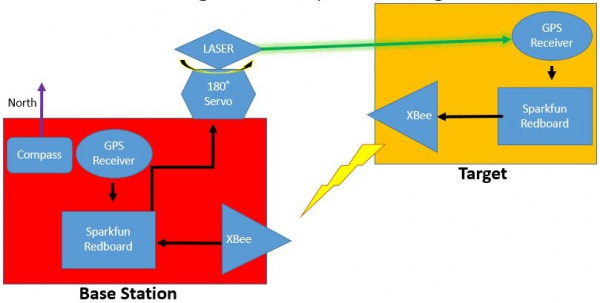
\includegraphics[scale=.3]{img/system}
\end{figure}

Verkefnið sem við ætlum að gera (Kjartan og Einar) er að búa til miðunartæki á milli 2 tækja með notkun GPS. Þetta getur verið notað til þess að miða t.d sensora, loftnetum, laserum o.sf frá einum object yfir á annan frá löngum vegalendum. Það verða tveir hlutir sem þarf að búa til, Base og Target (Það gæti samt verið hægt að nota síman sem target og við munum líta betur á það). Eina sem Target-ið á að gera er að fá GPS staðsetninguna á sjálfum sér, þátta gögnin frá því og senda það til baka á Base. Base mun þá fá upplýsingarnar um GPS-Staðsetninguna hjá Target og reiknar svo út frá sýnar eigin GPS Staðsetningu til að fá það sem kallast Positive Vector. Við munum nota forritið Arduino IDE fyrir kóðann sem þarf að innihalda eftirfarandi libraries : Software Serial, TinyGPS og Servo. Þetta verkefni hefur marga tilganga nú þegar í heiminum, eins og GPS í símum ef þú ert að reyna finna út hvernig þú kemst til Fjörðin í Hafnafirði, þá reiknar það út frá staðsetninguni þinni til staðsetninguna sem þú vilt fara og finnur út leiðina til að komast þangað fyrir þig, og það er líka notað til að finna og fylgjast með flugtæki og miðla. Oftast þegar þú kaupir svona GPS-reciever þá kostar það mun meira heldur en að búa bara til það sjálfur. Og ef eitthvað t.d týnist hjá þér, en það er með GPS-reciever á sér, geturu fundið það á mun stittri stund.
